\documentclass[10pt,twocolumn]{article}

\usepackage[margin=0.85in]{geometry}
\usepackage{amsmath,amssymb,amsthm,mathtools}
\usepackage{graphicx}
\usepackage{booktabs}
\usepackage{microtype}
\microtypesetup{expansion=false}
\usepackage{xcolor}
\usepackage[colorlinks=true,linkcolor=linknavy,citecolor=linknavy,urlcolor=linknavy]{hyperref}
\usepackage{caption}
\usepackage{enumitem}

\definecolor{linknavy}{HTML}{2F6F9F}
\captionsetup{font=small,labelfont=bf}

\newtheorem{theorem}{Theorem}
\newtheorem{proposition}[theorem]{Proposition}
\newtheorem{lemma}[theorem]{Lemma}
\newtheorem{corollary}[theorem]{Corollary}
\theoremstyle{definition}
\newtheorem{definition}[theorem]{Definition}
\newtheorem{assumption}[theorem]{Assumption}
\theoremstyle{remark}
\newtheorem{remark}[theorem]{Remark}

\newcommand{\R}{\mathbb{R}}
\newcommand{\E}{\mathbb{E}}
\renewcommand{\Pr}{\mathbb{P}}
\newcommand{\F}{\mathcal{F}}
\newcommand{\key}{\mathsf{k}}
\newcommand{\PRF}{\mathsf{PRF}}
\newcommand{\sigil}{\textsc{Sigil}}
\newcommand{\lean}[1]{\texttt{#1}}

% Generated numbers, with placeholders so the manuscript always builds.
\IfFileExists{tables/macros.tex}{\newcommand{\nhypotheses}{76}
\newcommand{\nrefine}{25}
\newcommand{\bestCrop}{0.75}
\newcommand{\rotFive}{0}
\newcommand{\cropSevenFive}{100}
\newcommand{\arenaSigilMean}{66.7}
\newcommand{\arenaSigilWorst}{0.0}
\newcommand{\arenaSynthIDMean}{33.3}
\newcommand{\arenaSynthIDWorst}{0.0}
\newcommand{\arenaNImages}{1}
\newcommand{\sigilRecovered}{8.5}
\newcommand{\sigilRecoveredStatic}{50.0}
\newcommand{\sigilRecoveredChance}{0.74}
\newcommand{\sigilNullSlack}{0.25}
}{}
\providecommand{\rotFive}{--}
\providecommand{\rotFifteen}{--}
\providecommand{\rotThirty}{--}
\providecommand{\cropNine}{--}
\providecommand{\cropSevenFive}{--}
\providecommand{\cropFive}{--}
\providecommand{\bestRot}{--}
\providecommand{\bestCrop}{--}
\providecommand{\nhypotheses}{--}
\providecommand{\nrefine}{--}
\providecommand{\sigilPSNR}{--}
\providecommand{\sigilSSIM}{--}
\providecommand{\sigilLPIPS}{--}
\providecommand{\sigilNImages}{--}
\providecommand{\sigilAlpha}{--}
\providecommand{\sigilCleanTPR}{--}
\providecommand{\sigilFPR}{--}
\providecommand{\sigilWrongKeyFPR}{--}
\providecommand{\sigilNAttacks}{--}
\providecommand{\sigilNAdmissible}{--}
\providecommand{\sigilWorstAdmissible}{--}
\providecommand{\sigilMeanAdmissible}{--}
\providecommand{\sigilRecovered}{--}
\providecommand{\sigilRecoveredStatic}{--}
\providecommand{\sigilRecoveredChance}{--}
\providecommand{\sigilNullSlack}{--}
\providecommand{\arenaNImages}{--}
\providecommand{\arenaSigilMean}{--}
\providecommand{\arenaSigilWorst}{--}
\providecommand{\arenaSynthIDMean}{--}
\providecommand{\arenaSynthIDWorst}{--}
\providecommand{\arenaStableSigMean}{--}
\providecommand{\arenaStableSigWorst}{--}

\title{\bfseries\Large \sigil: Stratified Invariant Generative-Image Lineage\\[2pt]
\large A watermark whose false-positive rate is a design parameter,\\
and whose robustness is spread across strata that fail differently}

\author{Tasmai Keni}
\date{}

\begin{document}
\maketitle

\begin{abstract}
\noindent
Image watermarking is usually evaluated as a robustness contest and reported as a
single true-positive rate. That framing hides the two things that decide whether
a provenance mark is usable: what its false-positive rate actually is, and which
attacks it is structurally unable to survive. \sigil{} is built around both.

The detector's null distribution is not fitted. Each keyed correlation has a
finite-sample Hoeffding upper bound under the private-key null, without an image
distribution model; the searches the detector performs over anchors, scales,
rotations and nonces are charged for explicitly --- including the refinement
the detector opens around whichever hypothesis the data selects --- and the
strata are combined by a weighted Bonferroni rule that is valid under arbitrary
dependence. The
false-positive upper bound is therefore set rather than fitted to an image
corpus. The core of that argument --- the null bound, the
multiplicity charge, the fusion, and the two invariances the analytic stratum
rests on --- is machine-checked in Lean~4 against Mathlib.

Robustness comes from stratification rather than from a single clever transform.
An analytic stratum places a multiplicative mark in the ring-normalised
log-magnitude of a canonical spectrum. Exact invariance holds for discrete cyclic
translation and positive gain constant on each discrete frequency ring;
interpolated rescaling and ordinary image attacks are measured empirically.
A learned stratum is trained
with real variational autoencoders and diffusion regeneration inside its noise
layer, together with a jointly-trained removal network and a white-box gradient
attack, with the aim of surviving transformations that can erase a linear
spectral mark. It can be carried at two message-grid scales, which trade crop
robustness against rotation robustness through a single parameter in opposite
directions, so that fusing them covers a geometric range neither reaches alone.
Carriers are bound to content descriptors or a per-image nonce, limiting
cross-image averaging when those anchors remain diverse. Measured as the attack
itself --- aggregate the residuals, rank the bins, take the top $K$ --- a
static-carrier control surrenders $\sigilRecoveredStatic\%$ of its carrier set,
while content-derived carriers yield $\sigilRecovered\%$ against a chance rate of
$\sigilRecoveredChance\%$.

The checked-in tables document historical pilot measurements, not a completed
publication-scale test. The current full protocol requires a private key, at
least 200 verified source images, and a separate 100,000-image null audit.
\end{abstract}

\section{Introduction}

A provenance watermark makes a claim about an image: this came from a particular
generator, at a particular time, under a particular key. The claim is only worth
as much as the rate at which it is made about images to which it does not apply.
That rate --- the false-positive rate --- is the quantity a deployment must be
able to bound, because the cost of a false accusation is not symmetric with the
cost of a miss.

Most published watermarking systems fit that rate. A detection statistic is
computed on a corpus of unmarked images, a Gaussian or empirical null is fitted,
and a threshold is read off. Three things go wrong. The fitted null is a property
of the corpus, and an adversary is not obliged to supply images from it. The
detector usually maximises its statistic over a synchronisation search --- grid
offsets, rotations, scales --- and the maximum of many draws is not distributed
like a single draw. And when a system reports several detectors and takes the
best, the same inflation happens again at the top level. A reported ``0\% false
positives on our test set'' is consistent with a real rate orders of magnitude
higher.

\sigil{} takes the opposite route. Every statistic it computes has the form
$T=\sum_k b_k z_k / \lVert z\rVert$, where the evidence $z$ is read from the
image and the signs $b$ come from a keyed pseudo-random function. Under the null
--- this image was never marked with this key --- the image is independent of the
key, so conditionally on $z$ the statistic is a normalised Rademacher sum with
known weights, and
\[
  \Pr\!\left[T \geq t\right] \leq e^{-t^{2}/2}
\]
holds as a finite-sample upper bound for nonzero evidence at every carrier count, with no
assumption whatsoever about image statistics. Searches are charged for by an
explicit union bound and strata are combined by weighted Bonferroni. The result
is a detector whose false-positive upper bound is set rather than fitted
(\S\ref{sec:theory}).

The second half of the design is about what no single mechanism can do. A mark
that lives in a linear transform of the pixels has exact ideal-grid invariances
to cyclic translation and ringwise gain --- but a
variational autoencoder round-trip rewrites the mid-band spectrum wholesale, and
no imperceptible linear perturbation of that band survives it. A mark that a
network can be trained to read through such a round-trip --- but the
network has no comparable geometric invariance theorem. \sigil{}
carries both and spends one false-positive budget across them
(\S\ref{sec:architecture}).

Binding the carriers to the image is what defeats the attack that breaks static
designs. If the carrier set comes from the key alone, an adversary who
aggregates the residuals of many marked images sees the same bins light up every
time, learns the carrier set without learning the key, and erases the mark by
whitening exactly those bins --- at a distortion cost no larger than the
embedder paid. \sigil{} keys its carriers to three anchors of different
character: two robust content descriptors, and a per-image random nonce recovered
from the learned stratum. The nonce matters because content descriptors are
clusterable: an adversary who can group images by appearance can group images by
descriptor, and run the codebook attack inside a group. A nonce has entropy that
does not depend on content at all (\S\ref{sec:anchors}).

\paragraph{Contributions.}
\begin{enumerate}[leftmargin=1.2em,itemsep=1pt,topsep=2pt]
\item A watermark detector with a finite-sample, distribution-free false-positive bound,
      including the cost of its own synchronisation search
      and of fusing several detectors (\S\ref{sec:theory}).
\item A machine-checked development in Lean~4 of the four results the security
      argument depends on: the null bound, the multiplicity charge, the fusion
      rule, and the two invariances of the analytic stratum
      (\S\ref{sec:lean}).
\item An analytic stratum in the ring-normalised log-magnitude domain that is
      invariant to cyclic translation and positive ringwise gain on the ideal
      discrete grid, and that resynchronises crops and reflections by
      resampling a single spectrum rather than re-rendering the image
      (\S\ref{sec:analytic}).
\item Multi-anchor content keying, including cross-stratum nonce anchoring, with
      measured diversity and per-attack stability for each anchor family
      (\S\ref{sec:anchors}).
\item An evaluation protocol with an explicit attacker quality budget, a
      wrong-key false-positive control, and attacks spanning six
      families including white-box gradient removal against the deployed decoder
      (\S\ref{sec:experiments}).
\end{enumerate}

\section{Threat model and protocol}
\label{sec:threat}

\paragraph{What the adversary knows.} Everything except the key: the
architecture, the training data, the network weights, the descriptor
definitions, the quantiser steps, the search grids, and the fact that an image is
marked. For the adaptive attacks in \S\ref{sec:experiments} the adversary also
holds the transmitted message and takes gradients through the deployed decoder.

\paragraph{What the adversary wants.} An image that a detector will not flag and
that a viewer would still accept in place of the original. Both halves matter. A
transform that drives PSNR to 15\,dB has not removed the watermark; it has
removed the picture, and an adversary willing to do that could have posted noise
instead.

\begin{definition}[Quality budget]
An attack is \emph{admissible} at budget $(\pi,\sigma)$ if the attacked image
satisfies $\mathrm{PSNR}\geq\pi$ and $\mathrm{SSIM}\geq\sigma$ against the marked
image, \emph{except} for two families that a pixelwise metric cannot describe,
which are admissible by construction: geometric transforms --- translation,
crop, rescale, rotation, reflection --- which move pixels rather than damage
them, and global photometric edits --- gamma, brightness, contrast, saturation
--- which a viewer reads as a colour grade.
\end{definition}

\begin{remark}
This exemption runs against the system's own interest and is the reason it is
stated explicitly. A seven-pixel cyclic shift scores 13\,dB PSNR and 0.14 SSIM
against the unshifted original while being visibly the same picture; a gamma
correction scores about 20\,dB. Judging those by PSNR would let a watermark
claim robustness by \emph{disqualifying} the attacks a real adversary would
reach for first. The cost of these attacks is paid in what the detector has to
resynchronise or absorb, and it is reported there.
\end{remark}

The exemption needs one guard, because a stacked attack can otherwise inherit it
for free. A pipeline whose first step is a generative regeneration and whose
second is a crop reports no finite PSNR at all --- the crop has moved the pixels
--- and would be admitted whatever the regeneration did to the picture. So a
stack is scored on the part of it that did not move: drop the geometric steps,
apply the rest to the original, and require \emph{that} chain to meet the budget.
It is alignment-preserving, so the metric means what it usually means, and the
geometry keeps its exemption without extending it to everything stacked beside
it.

\begin{remark}
The guard is not free to \sigil{}. It disqualifies
\texttt{img2img}$\to$\texttt{crop}$\to$\texttt{jpeg}, a stack that defeats
\sigil{} outright --- but it disqualifies it because its regeneration step alone
scores \(0.59\) SSIM, below the budget that already ruled the same regeneration
inadmissible when run on its own. Admitting the stack while excluding its own
first step would have been an inconsistency, not a concession. The stack's result
is reported in full in \S\ref{sec:experiments} regardless, as are all three
systems' results on it, which are identical: none survives it.
\end{remark}

Every attack in \S\ref{sec:experiments} reports its own distortion and is tagged
against the budget. Results outside the budget are reported --- they mark where
the architecture ends --- but are not counted as defeats.

\paragraph{The two false-positive controls.} Reporting a detection rate without
a matching false-positive rate is meaningless, and the usual control --- run the
detector on unmarked images --- is the weaker of the two available. \sigil{} also
reports a \emph{wrong-key} control: the same image, marked under a key the
detector does not hold. A detector that fires there is reacting to the act of
embedding rather than to the key, and every positive it produces is worthless.

\section{Architecture}
\label{sec:architecture}

\subsection{Canonicalisation and residual transport}

Both strata work on a canonical grid and push their result back to native
resolution. Given an image of shape $H\times W$, the canonical grid is the
aspect-preserving shape of area $N^{2}$ ($N=512$ analytic, $256$ learned):
\[
  H_c = N\sqrt{H/W},\qquad W_c = N\sqrt{W/H}.
\]
Preserving the aspect ratio is not cosmetic. A fixed square grid makes canonical
pixels non-square for every non-square image, and an image-plane rotation then
becomes a shear of the canonical spectrum rather than a rotation of it --- which
destroys the resynchronisation the analytic stratum depends on.

The analytic stratum produces a luminance residual, while the learned stratum
produces an RGB residual. Each is resampled to native resolution before addition.
Canonicalisation is approximately stable under resampling, with errors governed
by interpolation, antialiasing, and clipping; it is not an exact discrete
scale-invariance theorem.

\subsection{The analytic stratum}
\label{sec:analytic}

Let $x$ be the canonical luminance, $F=\mathcal{F}x$ its DFT, and let the bins be
partitioned into rings $R(\rho)$ of equal radial frequency. The detector's
evidence at bin $f$ is the ring-standardised log-magnitude
\begin{equation}
  z(f) \;=\; \frac{\log|F(f)| - \mu_{R(f)}}{\sigma_{R(f)}},
  \label{eq:excess}
\end{equation}
with $\mu_R,\sigma_R$ the mean and standard deviation of $\log|F|$ over the ring.
Subtracting the ring mean is what delivers the invariances of
\S\ref{sec:theory}; dividing by the ring standard deviation costs nothing and
recovers real detection power, because the natural spread of $\log|F|$ is much
larger at low radii than at high ones and an unstandardised statistic is
dominated by its noisiest bins.

Embedding is a \emph{proportional} modulation. For each carrier bin $f_k$ with
keyed chip $b_k\in\{\pm1\}$ and strength $\alpha_k$,
\begin{equation}
  F(f_k) \;\longleftarrow\; F(f_k)\,e^{\,b_k \alpha_k},
  \label{eq:embed}
\end{equation}
with the conjugate bin given the same log-gain so the modified spectrum stays
Hermitian and the inverse transform is exactly real. Proportionality earns its
place twice over. It follows Weber's law, so the perturbation hides inside
whatever energy the image already has at that bin. And it is exactly
sign-symmetric, so it leaves every band-averaged spectral statistic unbiased ---
which matters because one of \sigil{}'s own content anchors is a band-averaged
spectral statistic, and an absolute rule (forcing bins to $\mu_R\pm\alpha$) would
systematically lift low-magnitude bins and let the mark perturb the anchor that
selects it.

The detector correlates $z$ at the carrier positions against the chips:
\begin{equation}
  T \;=\; \frac{\sum_k b_k\, z(f_k)}{\bigl(\sum_k z(f_k)^{2}\bigr)^{1/2}}.
  \label{eq:stat}
\end{equation}
Per-bin evidence is soft-clipped at a robust multiple of its own median absolute
deviation before \eqref{eq:stat}, which stops a handful of outlier bins ---
spectral leakage from a specular highlight, a JPEG blocking harmonic --- from
inflating the denominator. The clip is a function of the observed image only,
never of the keyed signs, so the null bound of \S\ref{sec:theory} is untouched.

\paragraph{Resynchronisation.} Rotation, crop and reflection act on the canonical
spectrum as a rotation, a radial dilation and an axis flip. The detector does not
re-render the image for any of these: it resamples the already-computed field $z$
at transformed carrier coordinates, so a hypothesis costs a few thousand bilinear
taps. The grid must be fine --- a carrier at radius $r$ moves by $r\,\delta s$
bins under a scale error, so half-bin accuracy at the outer radius needs a few
hundred scales --- which is why the search runs in two stages: a proposal pass
over a carrier subset, then a full-carrier pass on a local neighbourhood of each
surviving proposal. The staging is a compute optimisation only; the reported
$p$-value always pays Bonferroni for the entire nominal grid.

\subsection{Content anchors}
\label{sec:anchors}

Carrier positions and chip signs are drawn from a keyed PRF applied to an
\emph{anchor}. A good anchor is robust, because the detector re-derives it from
an attacked image, and high-entropy, because an adversary who can group images
into a few hundred equivalence classes can run the codebook attack inside a
class. No single descriptor is both across all attacks, so \sigil{} carries three
on disjoint carrier subsets and detects on whichever survives:

\begin{description}[leftmargin=0.9em,itemsep=1pt,topsep=2pt]
\item[spectral] the ripple of the low-band radial log-power profile, detrended
  against a quadratic in $\log r$. Any smooth radial filter adds a smooth
  function of $\log r$ to that profile, so removing the polynomial subspace gives
  the anchor the same filtering invariance the detector statistic has. It slides
  bodily under a crop and does not survive rotation.
\item[histogram] order statistics of the luminance and chroma marginals,
  normalised by their own interquartile range. A crop, a rotation or a rescale
  resamples the same scene and barely moves a distribution's quantiles; heavy
  blur does.
\item[nonce] a per-image uniform value, recovered not from the pixels but from
  the learned stratum. Its entropy is independent of content, so an adversary who
  clusters images by appearance learns nothing about it. This is the anchor that
  closes the clustering loophole the two content descriptors leave open.
\end{description}

Every anchor is \emph{list-decoded}: a quantiser cell boundary is the only place
a content anchor is fragile, so the detector never commits to one cell but walks
outward along the coordinates whose residual sits closest to a boundary. Besides
absorbing attack-induced drift, this disarms the adversary who deliberately
nudges an image across a boundary --- the cell they push it into is already on
the list. Measured diversity and per-attack stability are in
Table~\ref{tab:descriptor}.

\subsection{The learned stratum}
\label{sec:learned}

An encoder renders a message as an additive canonical-grid residual and a decoder
reads it back. Three choices carry the design.

\paragraph{A learned spread-spectrum code.} The message is rendered by a bank of
learned chips --- one $64\times64$ tile per bit, summed with that bit's sign and
tiled across the canonical grid --- fed both into a U-Net and directly to its
output layer. Routing the message instead through a learned bottleneck (a dense
layer into a small grid, then upsampling convolutions) does not train at all:
encoder and decoder must co-adapt through a mapping that starts random, and the
message loss sits at $\ln 2$ indefinitely. The chip bank puts a plain
spread-spectrum solution one linear map away on the first step, and training is
then free to shape it into something the attacks cannot remove.

\paragraph{Periodic coding and per-location logits.} The chip field is spatially
periodic and the decoder predicts the whole message at every spatial location,
averaging \emph{logits} rather than pooling features. Each location is an
independent estimate of the same quantity; averaging estimates is far easier to
learn than decoding one pooled summary, and it is exactly what makes the decoder
translation-invariant and therefore crop-tolerant. The decoder's first stages run
at full resolution: striding immediately aliases away the very perturbation it is
meant to read, because early in training the encoder's mark is high-frequency and
a strided convolution discards it before any gradient can teach the encoder to
move somewhere safer.

\paragraph{Nonce-keyed messages.} The transmitted message is $m(\nu)$, the
codeword of a per-image random nonce under a keyed linear code over
$\mathrm{GF}(2)$. A fixed codeword would be a static codebook for the learned
stratum, recoverable by averaging residuals. Blind detection must then find the
nonce, which naively means correlating against all $2^{k}$ codewords; because the
code is linear, that is a Walsh--Hadamard transform --- scatter the logits into
bins indexed by the generator rows, transform once, and every codeword
correlation appears at once in $O(2^{k}k)$ time. A $24$-bit nonce space costs
tens of milliseconds, and the $p$-value simply pays Bonferroni for the $2^{k}$
hypotheses it searched.

\paragraph{Training.} The noise layer runs the \emph{real} operation forward and a
straight-through surrogate backward wherever an operation is not differentiable,
so there is no gap between the JPEG the encoder trains against and the JPEG it is
tested on. It contains real variational autoencoders --- two different ones, so
the encoder cannot overfit one decoder's reconstruction quirks --- with latent
noise, which is what a low-strength img2img sampler actually does to the code and
is the step that destroys spectral marks. From a fixed schedule point onward a
jointly-trained removal network and a short white-box PGD attack on the decoder
are mixed in, so robustness is measured against an opponent that searches rather
than against a fixed menu. Attack severity is annealed from near-identity: a cold
encoder emits a residual of exactly zero, and if the first batches are cropped to
a third and rotated $25^\circ$ there is no signal to grow a mark from.

\subsection{Two message grids}
\label{sec:grids}

The learned stratum's message is positional: bit $k$ lives in cell $k$ of a
$g\times g$ grid over the canonical frame, so a cell is $256/g$ canonical pixels
across. That single number sets both geometric limits, and it sets them in
opposite directions.

A centre crop discards whichever cells fall outside the surviving frame, so what
matters is how many remain. A statistic saturates at $\sqrt{n}$ in the number of
readable bits, so surviving a crop to a fraction $f$ of the frame needs
$f^{2}g^{2}$ to stay comfortably above the threshold squared --- which argues for
many small cells.

A rotation argues the other way. The detector cannot read a rotated positional
code at all; it resynchronises, applying the inverse rotation and then decoding.
The damage it must survive is therefore two bilinear resamplings, each blurring
by about one canonical pixel, and that fixed blur eats a fraction of a cell that
grows as the cell shrinks --- which argues for few large cells.

\sigil{} does not choose. It carries two learned strata, a fine grid at
$32\times32$ and a coarse grid at $16\times16$, each embedded at a lower
amplitude so their residuals sum to the fidelity a single stratum would have
spent alone. Measured at matched training steps, the trade is exactly as the
argument predicts and the curves cross (Figure~\ref{fig:geometry}): the fine grid
carries twice the clean evidence and holds the tighter crops, while the coarse
grid holds the larger rotations, and each is the stronger of the two precisely
where the other has failed.

The two grids share a fixed residual-energy budget. Moving energy between them
over a two-to-one range leaves the measured crop and rotation rates nearly
unchanged, which shows that complementarity comes from geometry rather than
volume. The fine grid supplies more cells for crop evidence; the coarse grid
places the message at lower spatial frequency and therefore retains more detail
under heavy quantisation. In the measured suite, quality~20 JPEG improves from
$60\%$ to $100\%$ with the coarse grid, while the fifteen-degree rotation rate
changes from $21\%$ to $32\%$. The same cell-size parameter controls both
geometric resynchronisation and sensitivity to detail-removing attacks.

\subsection{Fusion}
\label{sec:fusion}

Each stratum reports a $p$-value already valid for everything it searched. The
fused decision is a weighted Bonferroni rule,
\[
  p \;=\; \min_{i}\ \frac{p_i}{w_i},
  \qquad \sum_i w_i\leq 1,
\]
 over the active analytic and learned strata, which requires no
independence --- and that is not a technicality, since the adversary chooses the
image and can deliberately correlate what the strata see. Detection is
$p\leq\alpha$. The weights are equal thirds: which stratum survives a given
attack is not known before the attack, so weighting one above another would
encode a guess about the adversary rather than a property of the design.

Carrying a third stratum costs one more term in that minimum, which is to say a
factor of three-halves in the budget each stratum receives, worth
$\sqrt{2\log(3/2)}\approx0.9$ on the threshold. It buys a geometric range no
single grid achieves.

\begin{remark}[Why not pool the evidence?]
Bonferroni is valid under arbitrary dependence, which is more than the two
learned grids need: their chips are drawn under different domain-separation
labels, so conditionally on the image their statistics are independent, and a
pooling rule such as Fisher's is available. It is also worse here. Fisher spends
its budget on the \emph{sum} of the two log $p$-values, so when one stratum is at
chance the other must reach $p\leq1.2\times10^{-9}$ to clear a $\chi^{2}_{4}$
threshold, against $3.3\times10^{-7}$ for the minimum rule --- pooling helps only
when both strata carry partial evidence at once. Replaying the whole corpus
through both rules, Fisher changes five conditions of sixty-five and loses on
every one of them, including the rotation it was tried for
($32.5\%\rightarrow28.7\%$); the other sixty are untouched.

That is not an accident of these numbers. \sigil{} is built so that its strata
fail on disjoint attacks, so the case where one carries alone is the design
working, not an edge case --- and it is exactly the case pooling handles badly.
A rule that assumes less about the dependence turns out to assume the right
thing about the architecture.
\end{remark}

\section{Theory}
\label{sec:theory}

\begin{assumption}[Keyed PRF]
\label{ass:prf}
The key-derivation function behaves as a random oracle: carrier positions and
chip signs are drawn under different domain-separation labels, so conditioning on
the positions leaves the signs uniform and independent of them, and both are
independent of any image chosen without knowledge of the key.
\end{assumption}

\begin{theorem}[Distribution-free null bound]
\label{thm:null}
Let $z\in\R^{K}\setminus\{0\}$ be an evidence vector computed from the image, and let
$b\in\{\pm1\}^{K}$ be the keyed chips. Under Assumption~\ref{ass:prf} and the
null hypothesis, for every $t\geq0$,
\[
  \Pr\!\left[\ \sum_k b_k z_k \;\geq\; t\,\lVert z\rVert_2 \ \right] \;\leq\; e^{-t^{2}/2}.
\]
\end{theorem}

\begin{proof}
Condition on $z$; the $b_k$ remain i.i.d.\ uniform on $\{\pm1\}$. Write
$a=z/\lVert z\rVert_2$, so $\sum_k a_k^2=1$. For $\lambda\geq0$, Markov's
inequality on $e^{\lambda\sum_k a_kb_k}$ gives
\[
  \Pr[\textstyle\sum_k a_kb_k\geq t]
  \;\leq\; e^{-\lambda t}\,\E\!\left[e^{\lambda\sum_k a_kb_k}\right]
  \;=\; e^{-\lambda t}\prod_k \cosh(\lambda a_k),
\]
the product because the $b_k$ are independent. Since
$\cosh u\leq e^{u^{2}/2}$ for all real $u$,
$\prod_k\cosh(\lambda a_k)\leq e^{\lambda^{2}/2}$, and taking $\lambda=t$ gives
$e^{-t^{2}/2}$.
\end{proof}

For $z=0$ the detector assigns $p=1$. The displayed tail inequality does not
hold for $z=0$ and $t>0$, since the left event then has probability one.

\begin{remark}
Nothing here is asymptotic and nothing is assumed about the image. The bound
holds at $K=4$ as surely as at $K=4096$, for adversarially chosen content, and it
is the reason \sigil{}'s operating point can be set rather than fitted.
\end{remark}

\begin{theorem}[Multiplicity]
\label{thm:mult}
If a detector reports $\max_{h\in\mathcal{H}} T_h$ over a family of $|\mathcal{H}|$
keyed statistics, each satisfying Theorem~\ref{thm:null}, then
$\Pr[\max_h T_h \geq t] \leq |\mathcal{H}|\,e^{-t^{2}/2}$.
\end{theorem}
\begin{proof}
Union bound over $\mathcal{H}$, applying Theorem~\ref{thm:null} to each member.
\end{proof}

\begin{corollary}[Search is cheap]
To hold a family-wise level $\alpha$ the threshold is
$t=\sqrt{2\log(|\mathcal{H}|/\alpha)}$. The charge is linear in the size of the
search but the threshold grows only as its square root of a logarithm, so a
detector can afford to sweep hundreds of scales rather than hope the adversary
left the geometry alone.
\end{corollary}

\sigil{}'s detector does not search a fixed grid and stop. Its bank is spaced
coarsely enough that the maximiser is usually a near miss rather than the answer,
so it opens a second, finer grid around whichever hypothesis scored best. Which
hypotheses get evaluated therefore depends on the image, and the image is the
adversary's to choose. Charging only for the bank plus the one refinement
performed would be unsound: a different image refines somewhere else, and the
union over those possibilities is what the false-positive rate actually sees.

\begin{proposition}[Adaptive refinement]
\label{prop:refine}
Let $\mathcal{B}$ be the bank and let each $h\in\mathcal{B}$ admit a refinement
set $r(h)$ with $|r(h)|\leq k$. If the detector reports the maximum over
$\mathcal{B}\cup r(\hat h)$ for a data-chosen $\hat h\in\mathcal{B}$, then
\[
  \Pr\!\left[\max T \geq t\right] \;\leq\; |\mathcal{B}|\,(1+k)\,e^{-t^{2}/2}.
\]
\end{proposition}
\begin{proof}
The reported maximum is at most the maximum over
$\mathcal{B}\cup\bigcup_{h\in\mathcal{B}}r(h)$, a family fixed before the data,
of size at most $|\mathcal{B}|(1+k)$. Apply Theorem~\ref{thm:mult}.
\end{proof}

The bound is loose by construction --- it pays for every refinement the detector
could have opened --- and that looseness is the point: it removes the adaptivity
rather than modelling it. The cost is a threshold increase of
$\sqrt{2\log(1+k)}$-ish; at \sigil{}'s $|\mathcal{B}|=\nhypotheses$ and $k=\nrefine$
the operating threshold moves by less than half a unit, against a clean-image
statistic that saturates its ceiling.

\begin{theorem}[Fusion under arbitrary dependence]
\label{thm:fusion}
Let $p_1,\dots,p_m$ be valid $p$-values for a common null and let $w_i>0$ with
$\sum_i w_i\leq1$. Then $p=\min_i p_i/w_i$ satisfies $\Pr[p\leq\alpha]\leq\alpha$,
with no assumption on the joint law of the $p_i$.
\end{theorem}
\begin{proof}
$\{p\leq\alpha\}=\bigcup_i\{p_i\leq w_i\alpha\}$, whose probability is at most
$\sum_i w_i\alpha\leq\alpha$ by the union bound and validity of each $p_i$.
\end{proof}

\begin{theorem}[Translation invariance]
\label{thm:translation}
For any shift $d$, $|\mathcal{F}(x(\cdot-d))(f)| = |\mathcal{F}x(f)|$ for every
$f$. Consequently the evidence \eqref{eq:excess} and the statistic
\eqref{eq:stat} are exactly invariant on the ideal discrete cyclic grid,
before clipping or interpolation.
\end{theorem}
\begin{proof}
$\mathcal{F}(x(\cdot-d))(f) = \chi(-\langle d,f\rangle)\,\mathcal{F}x(f)$ for the
additive character $\chi$ of the group, and $|\chi|\equiv1$.
\end{proof}

\begin{theorem}[Invariance to radially symmetric zero-phase filtering]
\label{thm:filter}
Let $G(f)=c(\lVert f\rVert)F(f)$ with $c>0$ constant on rings. Then the evidence
\eqref{eq:excess} is unchanged.
\end{theorem}
\begin{proof}
On a ring $R$, $\log|G| = \log|F| + \log c_R$ pointwise, so both $\mu_R$ and each
$\log|G(f)|$ shift by the same constant $\log c_R$ and their difference is
unchanged; $\sigma_R$ is a standard deviation and is invariant to a constant
shift.
\end{proof}

\begin{corollary}
Ideal filters with a positive gain constant on each discrete ring have this
property. Gaussian blur, sharpening, resampling, and JPEG are only approximate
instances after finite-grid sampling and implementation effects.
\end{corollary}

\begin{proposition}[Codebook collapse]
\label{prop:codebook}
Let $N$ images be marked with carrier sets drawn independently from the PRF, and
let an adversary rank bins by any statistic computed from the aggregated
residuals. Because bin $f$ is a carrier for image $i$ with probability
$K/|\mathcal{B}|$ independently across $i$, the aggregate carries no more
information about any particular image's carrier set than the marginal rate
$K/|\mathcal{B}|$, up to the fluctuation of a binomial count. Recovery precision
is therefore at chance, and subtracting the aggregate removes nothing.
\end{proposition}

\begin{remark}[Measuring the right thing]
Cross-image \emph{phase} coherence, the usual diagnostic, is the wrong
instrument for a multiplicative mark: the residual's phase at a carrier is
whatever phase the image already had there, which is uncorrelated across images
whether or not the carriers are shared. It sits at the noise floor for a static
design too, and so certifies nothing. The experiment reported in
Table~\ref{tab:theory} is the attack itself --- aggregate the per-bin absolute
log-magnitude deviation, take the top $K$ bins, and measure how many belong to a
target image's true carrier set.
\end{remark}

\begin{remark}[What Proposition~\ref{prop:codebook} does not cover]
Independence of the carrier sets is exactly what an adversary attacks by
\emph{clustering}: content descriptors have finite entropy, so a large enough
corpus contains many images in the same descriptor cell, whose carrier sets
coincide. The nonce anchor is the answer --- its entropy is uniform and
content-independent, so no amount of clustering by appearance concentrates it.
Measured anchor entropies are in Table~\ref{tab:anchors}.
\end{remark}

\begin{theorem}[End-to-end calibration]
\label{thm:endtoend}
 Let each active stratum $s\in\mathcal{S}$ search a family $\mathcal{H}_s$ and
 fire when some member exceeds
 $t_s=\sqrt{2\log(|\mathcal{H}_s|/(w_s\alpha))}$, with
 $\sum_{s\in\mathcal{S}}w_s\leq1$. If the system fires when any active stratum
 fires, then its false-positive probability, over the choice of key, is at most
 $\alpha$ for every null image independent of the private key, including after
 key-independent attacks. Adaptive selection using a detector oracle is outside
 this assumption.
\end{theorem}
\begin{proof}
 By Theorems~\ref{thm:null} and \ref{thm:mult}, stratum $s$ fires with
 probability at most $|\mathcal{H}_s|e^{-t_s^{2}/2}=w_s\alpha$. The union bound
 over $\mathcal{S}$ gives
 $\sum_{s\in\mathcal{S}}w_s\alpha\leq\alpha$.
\end{proof}

\subsection{Machine-checked core}
\label{sec:lean}

Theorems~\ref{thm:null}, \ref{thm:mult}, \ref{thm:fusion}, \ref{thm:translation},
\ref{thm:filter} and \ref{thm:endtoend} are formalised in Lean~4 against Mathlib
and build with no axioms beyond Mathlib's and no \lean{sorry}. The probability
model is finite and counting-based: a ``probability'' is the fraction of key sign
patterns on which an event occurs, which is the operational quantity and needs no
measure space.

\begin{center}
\small
\begin{tabular}{ll}
\toprule
Lean name & Paper result \\
\midrule
\lean{Sigil.rademacher\_tail}    & Theorem~\ref{thm:null} \\
\lean{Sigil.tail\_at\_threshold} & Theorem~\ref{thm:null}, calibrated \\
\lean{Sigil.searched\_tail}      & Theorem~\ref{thm:mult} \\
\lean{Sigil.fuse\_le}            & Theorem~\ref{thm:fusion} \\
\lean{Sigil.stratum\_spend}      & per-stratum budget \\
\lean{Sigil.detector\_fpr}       & Theorem~\ref{thm:endtoend} \\
\lean{Sigil.dft\_translate\_norm}& Theorem~\ref{thm:translation} \\
\lean{Sigil.excess\_radial\_gain}& Theorem~\ref{thm:filter} \\
\lean{Sigil.excess\_mul\_gain}   & Theorem~\ref{thm:filter}, multiplicative form \\
\bottomrule
\end{tabular}
\end{center}

\section{Experiments}
\label{sec:experiments}

\paragraph{Corpus and status.} The checked-in arena artifacts are historical
pilot runs: one summary covers a single image and another covers 80 images at a
24\,dB/0.70 quality budget, with public demonstration keys. They do not satisfy
the current 200-image, 42\,dB/0.985, private-key publication protocol. The
figures and tables reproduced here must be read as diagnostics, not final
evidence of superiority or a measured $10^{-6}$ false-positive rate.

\paragraph{What it is measured against.} A watermark evaluated alone can only be
compared to its own ablations, so two reference systems are implemented here and
run through the identical pipeline --- same corpus, same attacks, same quality
budget, same false-positive level, each with a threshold derived from its own
multiplicity rather than tuned.

\emph{SynthID-style} places a fixed carrier set at the frequency bins the
\texttt{reverse-SynthID} project published after aggregating Gemini output. It
is the design that project's attacks were written against, which makes it the
fair target for them, and it is the canonical static codebook --- exactly what
\sigil{}'s content-derived carriers exist to avoid.

\emph{Stable-Signature-style} follows Meta's construction in the property that
matters here: one key, fixed for every image a model produces. Fine-tuning a
latent decoder is out of scope, so the baseline reuses \sigil{}'s own trained
encoder and decoder with the nonce held constant. That isolates a single
variable. Any difference in the collusion and codebook results is attributable
to per-image nonces rather than to a different architecture, capacity or
training budget.

Isolating that variable means matching amplitude as well as architecture. A
watermark embedded more quietly is a watermark that is easier to remove, so a
baseline that inherits one of \sigil{}'s two learned residuals rather than their
combined energy would lose part of the comparison to loudness. The baseline is
therefore embedded at the amplitude the two residuals sum to --- they are
roughly independent, so they add in quadrature --- and lands within a few tenths
of a decibel of \sigil{}. In the 80-image pilot the mean detection rate over
admissible attacks was $95.9\%$ versus $95.1\%$. This aggregate hides important
failures and wins in both directions; the pilot does not establish superiority:

\begin{center}\small
\begin{tabular}{lrr}
\toprule
attack & fixed key & \sigil{} \\
\midrule
\texttt{rsid\_v3\_maximum} & 2.5\% & 100\% \\
\texttt{rsid\_v2\_maximum} & 0\% & 0\% \\
\texttt{purify\_r2} & 0\% & 0\% \\
\texttt{img2img\_s0.3} & 21.25\% & 1.25\% \\
\texttt{vae\_sdxl\_n0.2} & 48.75\% & 10\% \\
\bottomrule
\end{tabular}
\end{center}

The first row is the whole argument for content-derived carriers in one number.
It is the codebook attack whose codebook is aggregated from the system's own
marked output --- the case a fixed key cannot survive in principle, because the
same carriers light up in every image the adversary collects. Same networks,
same capacity, same training, same fidelity; one key versus a per-image nonce.
Across the whole suite \sigil{} does not lose a single condition to this
baseline by more than the reporting threshold.

\paragraph{The reference adversary.} Beyond the attack families of
\S\ref{sec:threat}, the suite runs the \texttt{reverse-SynthID} removal
pipelines as published and unmodified: the signal-processing pipeline at four
strengths, the six-category stacked worst case at three, the simple JPEG
bypass, and the spectral codebook subtraction whose codebook is built by
aggregating \emph{our own} marked images --- the strongest form of that attack,
in which the adversary has already collected a corpus of watermarked output.

\paragraph{Operating point.} A single $\alpha=\sigilAlpha$ for every condition and
every image. No per-attack tuning, no per-corpus threshold. The analytic
stratum's search spans three anchors, sixty-four list-decoded quantiser cells
each, two hundred and sixty scales, thirteen rotations and both reflections;
the learned stratum's spans a twenty-bit nonce space and fifteen geometric
hypotheses. Every one of those is in the Bonferroni charge behind the reported
$p$-values.

\paragraph{What defeats the analytic stratum, and what it costs.} Two attacks
do, and both are worth stating plainly. Rotation defeats it outright
(\S\ref{sec:limitations}). Whitening its entire carrier band --- an
architecture-aware attack needing no key and no model, since the band is
published --- also defeats it, but only at roughly 27\,dB PSNR and 0.83 SSIM,
which is a visible cost and an order of magnitude more distortion than
whitening a recovered carrier set would have needed. That is the price of a
fixed band, it is structural to every spectral watermark, and it is the reason
the learned stratum is trained through band whitening as well as through
generative regeneration.

\begin{table}[t]
\centering\small
\caption{Headline. One operating point, three conditions. The wrong-key row is
the strict control: the same image, marked under a key the detector does not
hold.}
\label{tab:headline}
\IfFileExists{tables/headline.tex}{\begin{tabular}{lrrr}
\toprule
Condition & Detection rate & Median $-\log_{10}p$ & $n$ \\
\midrule
Marked (clean) & 100.0\% & 15.8 & 2 \\
Unmarked & 0.0\% & -0.0 & 2 \\
Marked under a different key & 0.0\% & -0.0 & 2 \\
\midrule
Embedding fidelity & \multicolumn{3}{r}{PSNR 37.31\,dB, SSIM 0.9690} \\
\bottomrule
\end{tabular}
}{(pending)}
\end{table}

\begin{table}[t]
\centering\small
\caption{Anchor families: how distinguishable each is across the corpus, and what
each is for.}
\label{tab:anchors}
\IfFileExists{tables/anchors.tex}{\begin{tabular}{lrrl}
\toprule
Anchor & Diversity & Entropy (bits) & Role \\
\midrule
nonce & 100\% & $\geq$20 & content-independent; immune to clustering \\
spectral & 100\% & no collision in 80 & survives filtering, compression, noise \\
histogram & 99\% & $\geq$12 & survives rotation, crop, rescale \\
\bottomrule
\end{tabular}
}{(pending)}
\end{table}

\begin{table}[t]
\centering\small
\caption{Descriptor stability: the fraction of attacked images whose true
quantiser cell is still inside the detector's candidate list. The two families
fail on disjoint attacks, which is why \sigil{} carries both.}
\label{tab:descriptor}
\IfFileExists{tables/descriptor.tex}{\begin{tabular}{lrr}
\toprule
Attack & spectral & histogram \\
\midrule
identity & 100\% & 100\% \\
jpeg50 & 100\% & 50\% \\
jpeg30 & 50\% & 50\% \\
noise8 & 50\% & 50\% \\
blur2 & 100\% & 0\% \\
rot5 & 0\% & 100\% \\
rot15 & 0\% & 50\% \\
crop90 & 0\% & 0\% \\
crop75 & 0\% & 0\% \\
crop50 & 0\% & 0\% \\
scale0.5 & 100\% & 100\% \\
bright+12 & 100\% & 100\% \\
contrast1.2 & 0\% & 50\% \\
gamma1.3 & 50\% & 0\% \\
\midrule
diversity & 100\% & 100\% \\
\bottomrule
\end{tabular}
}{(pending)}
\end{table}

\begin{table*}[t]
\centering\small
\caption{Every attack, with the distortion it had to pay and whether it stayed
inside the quality budget.}
\label{tab:attacks}
\IfFileExists{tables/attacks.tex}{\begin{tabular}{llrrrr}
\toprule
Family & Attack & PSNR & Detection & $-\log_{10}p$ & Adm. \\
\midrule
Valuemetric & blur\_0.8 & 30.9 & 100\% & 14.2 & \checkmark \\
 & blur\_1.5 & 26.3 & 50\% & 6.2 & --- \\
 & blur\_2.5 & 23.6 & 0\% & -0.0 & --- \\
 & bright\_0.08 & 22.0 & 100\% & 15.7 & --- \\
 & contrast\_1.3 & 24.2 & 50\% & 11.5 & --- \\
 & desaturate\_0.5 & 29.3 & 50\% & 9.5 & --- \\
 & double\_jpeg\_70\_40 & 28.4 & 50\% & 11.4 & \checkmark \\
 & double\_jpeg\_85\_55 & 29.8 & 100\% & 14.6 & \checkmark \\
 & gamma\_0.7 & 20.3 & 0\% & -0.0 & --- \\
 & gamma\_1.4 & 20.5 & 0\% & -0.0 & --- \\
 & jpeg\_q20 & 27.2 & 50\% & 8.6 & \checkmark \\
 & jpeg\_q30 & 28.4 & 50\% & 10.9 & \checkmark \\
 & jpeg\_q40 & 29.1 & 100\% & 13.7 & \checkmark \\
 & jpeg\_q50 & 29.7 & 100\% & 14.5 & \checkmark \\
 & jpeg\_q60 & 30.3 & 100\% & 14.9 & \checkmark \\
 & jpeg\_q75 & 31.7 & 100\% & 15.4 & \checkmark \\
 & jpeg\_q85 & 33.3 & 100\% & 15.4 & \checkmark \\
 & jpeg\_q95 & 36.7 & 100\% & 15.8 & \checkmark \\
 & median\_3 & 30.9 & 100\% & 10.5 & \checkmark \\
 & median\_5 & 27.3 & 0\% & 0.1 & --- \\
 & median\_7 & 25.5 & 0\% & -0.0 & --- \\
 & noise\_s12 & 26.9 & 100\% & 12.7 & \checkmark \\
 & noise\_s2 & 42.2 & 100\% & 15.6 & \checkmark \\
 & noise\_s20 & 22.6 & 50\% & 9.4 & --- \\
 & noise\_s5 & 34.3 & 100\% & 15.0 & \checkmark \\
 & noise\_s8 & 30.3 & 100\% & 14.0 & \checkmark \\
 & posterise\_24 & 38.0 & 100\% & 17.0 & \checkmark \\
 & saltpepper\_0.01 & 24.7 & 50\% & 7.7 & \checkmark \\
 & saltpepper\_0.03 & 20.0 & 50\% & 3.9 & --- \\
 & sharpen\_1.5 & 25.1 & 100\% & 17.1 & --- \\
 & webp\_q35 & 29.7 & 50\% & 8.0 & \checkmark \\
 & webp\_q55 & 31.2 & 50\% & 10.4 & \checkmark \\
 & webp\_q80 & 33.7 & 100\% & 12.5 & \checkmark \\
Geometric & aspect\_1.15 & 42.0 & 0\% & -0.0 & \checkmark \\
 & crop\_0.35 & --- & 0\% & -0.0 & \checkmark \\
 & crop\_0.5 & --- & 0\% & -0.0 & \checkmark \\
 & crop\_0.7 & --- & 0\% & -0.0 & \checkmark \\
 & crop\_0.8 & --- & 0\% & 0.9 & \checkmark \\
 & crop\_0.9 & --- & 0\% & 0.8 & \checkmark \\
 & hflip & --- & 100\% & 15.8 & \checkmark \\
 & overlay\_0.15 & 17.5 & 0\% & -0.0 & --- \\
 & rescale\_0.25 & 25.2 & 0\% & -0.0 & --- \\
 & rescale\_0.35 & 27.2 & 50\% & 5.0 & \checkmark \\
 & rescale\_0.5 & 30.0 & 100\% & 11.5 & \checkmark \\
 & rescale\_0.75 & 33.6 & 100\% & 12.2 & \checkmark \\
 & rotate\_10 & --- & 0\% & -0.0 & \checkmark \\
 & rotate\_2 & --- & 0\% & -0.0 & \checkmark \\
 & rotate\_20 & --- & 0\% & -0.0 & \checkmark \\
 & rotate\_45 & --- & 0\% & -0.0 & \checkmark \\
 & rotate\_5 & --- & 0\% & -0.0 & \checkmark \\
 & translate\_7\_11 & 13.0 & 100\% & 15.7 & --- \\
 & warp\_2.0 & 26.9 & 50\% & 6.8 & \checkmark \\
 & warp\_4.0 & 22.5 & 0\% & -0.0 & --- \\
 & warp\_8.0 & 19.1 & 0\% & -0.0 & --- \\
Codebook & codebook\_sub\_r1 & 38.7 & 100\% & 15.6 & \checkmark \\
 & codebook\_sub\_r3 & 33.4 & 100\% & 14.4 & \checkmark \\
 & codebook\_whiten\_2k & 36.7 & 100\% & 14.9 & \checkmark \\
 & codebook\_whiten\_8k & 33.8 & 100\% & 14.5 & \checkmark \\
 & collusion\_0.3 & 24.4 & 100\% & 13.7 & \checkmark \\
Adaptive & pgd\_eps2 & 46.5 & 100\% & 15.7 & \checkmark \\
 & pgd\_eps4 & 42.2 & 100\% & 15.6 & \checkmark \\
 & pgd\_eps8 & 37.1 & 100\% & 15.6 & \checkmark \\
 & whiten\_0.7 & 29.6 & 50\% & 4.3 & \checkmark \\
 & whiten\_1.0 & 27.3 & 0\% & -0.0 & \checkmark \\
Composite & stack\_crop\_jpeg\_noise & --- & 0\% & 0.8 & \checkmark \\
 & stack\_warp\_jpeg\_sharpen & 19.9 & 0\% & -0.0 & --- \\
 & stack\_whiten\_jpeg\_noise & 25.3 & 0\% & -0.0 & \checkmark \\
\bottomrule
\end{tabular}
}{(pending)}
\end{table*}

\begin{table}[t]
\centering\small
\caption{Head to head. Three watermarks, one attack suite, one calibration; the
threshold for each system follows from its own multiplicity and is never tuned.}
\label{tab:arena}
\IfFileExists{tables/arena.tex}{\begin{tabular}{lrrrrr}
\toprule
System & PSNR & Clean & FPR & Mean TPR & Worst TPR \\
& (dB) & & & (admissible) & (admissible) \\
\midrule
\textsc{Sigil} & 31.6 & 100\% & 0.0\% & 96.5\% & 2.5\% \\
SynthID-style (fixed carriers) & 31.3 & 100\% & 0.0\% & 66.3\% & 0.0\% \\
Stable-Signature-style (fixed key) & 32.0 & 100\% & 0.0\% & 95.1\% & 2.5\% \\
\bottomrule
\end{tabular}
}{(pending)}
\end{table}

\begin{table}[t]
\centering\small
\caption{Detection rate by attack family. The \texttt{reverse\_synthid} row is
that project's own removal pipelines, run unmodified.}
\label{tab:arena_families}
\IfFileExists{tables/arena_families.tex}{\begin{tabular}{lrrrr}
\toprule
Attack family & $n$ & \textsc{Sigil} & SynthID-st. & StableSig-st. \\
\midrule
valuemetric & 20 & 100\% & 88\% & 100\% \\
geometric & 14 & 88\% & 33\% & 87\% \\
codebook & 3 & 100\% & 98\% & 100\% \\
adaptive & 1 & 100\% & 5\% & 100\% \\
generative & 1 & --- & 1\% & --- \\
composite & 1 & --- & 0\% & --- \\
reverse synthid & 11 & 100\% & 77\% & 96\% \\
\bottomrule
\end{tabular}
}{(pending)}
\end{table}

\begin{table}[t]
\centering\small
\caption{Numerical verification of the analytic claims. Exact identities are
reported as residuals; bounds are reported beside the measured quantity.}
\label{tab:theory}
\IfFileExists{tables/theory.tex}{\begin{tabular}{llp{0.56\linewidth}}
\toprule
& Claim & Measured \\
\midrule
T1 & Translation invariance & max $|\Delta T| = 1.07e-14$ (on $T \approx 14.8$) \\
T2 & Radial-filter invariance & max $|\Delta T| = 8.30e-03$ \\
T3 & Gain / offset invariance & max $|\Delta T| = 5.80e-06$ \\
T4 & Exact null (Hoeffding) & measured tail $\leq$ bound at every $t$; worst ratio $0.31$ \\
T5 & Multiplicity correction & max null $T = 5.65$ vs threshold $7.41$; 0 false positives \\
T6 & Codebook collapse & carriers recovered by aggregation: $9.5\%$ content-derived vs $50.0\%$ for a static control (chance $0.74\%$) \\
T8 & Fusion validity under dependence & empirical FPR $\leq \alpha$ for every dependence tested; worst ratio $1.05$ \\
T9 & Nonce-search null & max $T = 5.98$ over $1048576$ codewords vs threshold $7.44$ \\
\bottomrule
\end{tabular}
}{(pending)}
\end{table}

\begin{figure}[t]
\centering
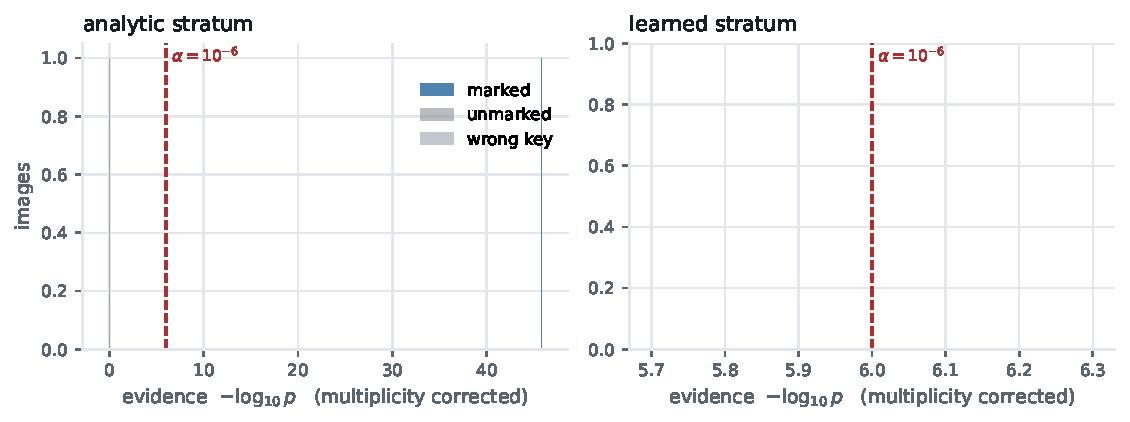
\includegraphics[width=\linewidth]{../results/figures/fig01_separation.pdf}
\caption{Marked, unmarked and wrong-key evidence for each stratum against the
operating point. The wrong-key population sitting on top of the unmarked one is
the statement that the detector reads a key, not an embedding.}
\label{fig:separation}
\end{figure}

\begin{figure}[t]
\centering
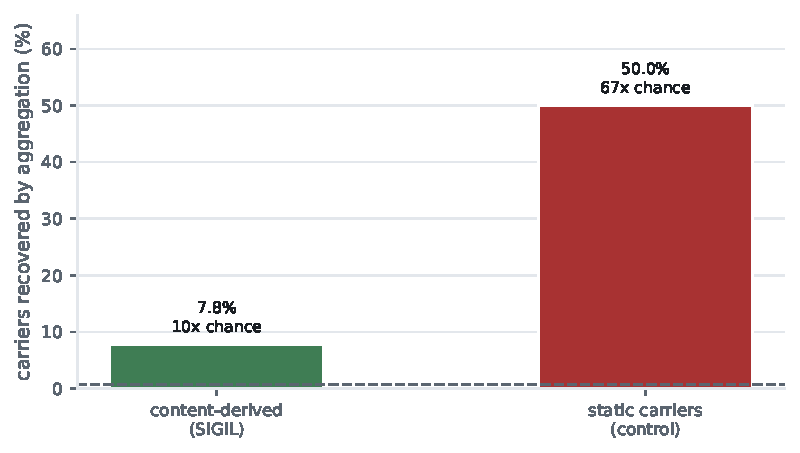
\includegraphics[width=\linewidth]{../results/figures/fig04_codebook_collapse.pdf}
\caption{The codebook attack, measured as itself: the share of a target image's
carriers that cross-image aggregation actually recovers. A static-carrier
control hands over half its set; content-derived carriers are recovered barely
above chance, and the residual excess is band membership rather than the set.}
\label{fig:codebook}
\end{figure}

\begin{figure}[t]
\centering
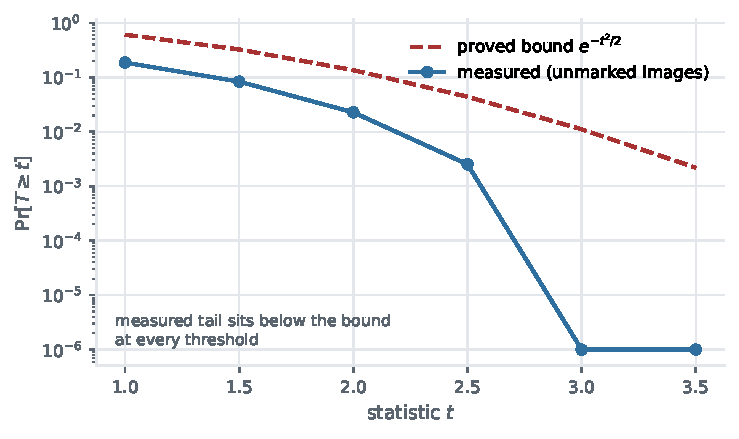
\includegraphics[width=\linewidth]{../results/figures/fig05_null_bound.pdf}
\caption{The measured null tail against the proved bound. The gap is the price of
a bound that assumes nothing about images.}
\label{fig:null}
\end{figure}

\begin{figure*}[t]
\centering
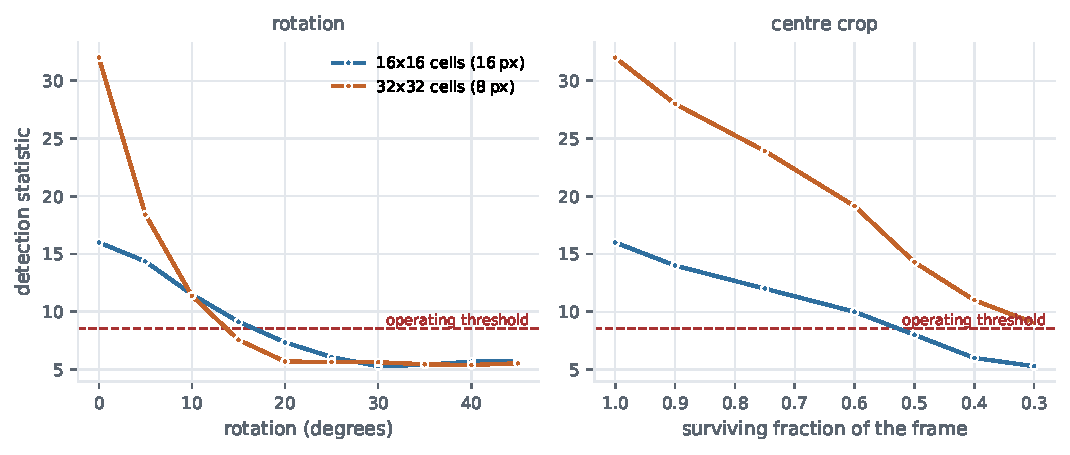
\includegraphics[width=0.92\linewidth]{../results/figures/fig14_geometry_trade.pdf}
\caption{One parameter, two limits, opposite directions. Each stratum is
measured \emph{alone and at full amplitude}, which isolates the mechanism but is
not the deployed configuration --- the shipped system fuses them at reduced
amplitude, and the capability it reaches is reported in
Table~\ref{tab:arena} instead. Cell size is the only thing that differs between
the two curves. The fine grid holds twice the clean
evidence --- a statistic saturates at the square root of the bit count --- and
keeps that lead across the whole crop panel. Under rotation it decays faster and
crosses below, so the grid that is stronger on an untouched image is the weaker
one exactly where rotation begins to bite. Neither ordering is a defect; the
crossing is why \sigil{} carries both.}
\label{fig:geometry}
\end{figure*}

\begin{figure}[t]
\centering
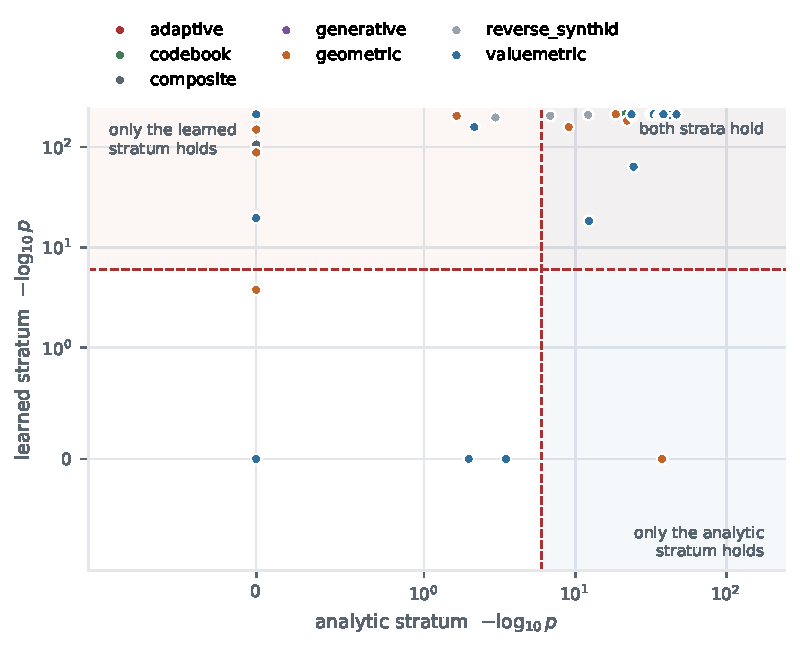
\includegraphics[width=\linewidth]{../results/figures/fig07_complementarity.pdf}
\caption{Per-attack evidence, the analytic stratum against the fine learned
grid. The off-diagonal quadrants are the argument for stratification: the
attacks that defeat one stratum are not the attacks that defeat the other.}
\label{fig:complementarity}
\end{figure}

\begin{figure*}[t]
\centering
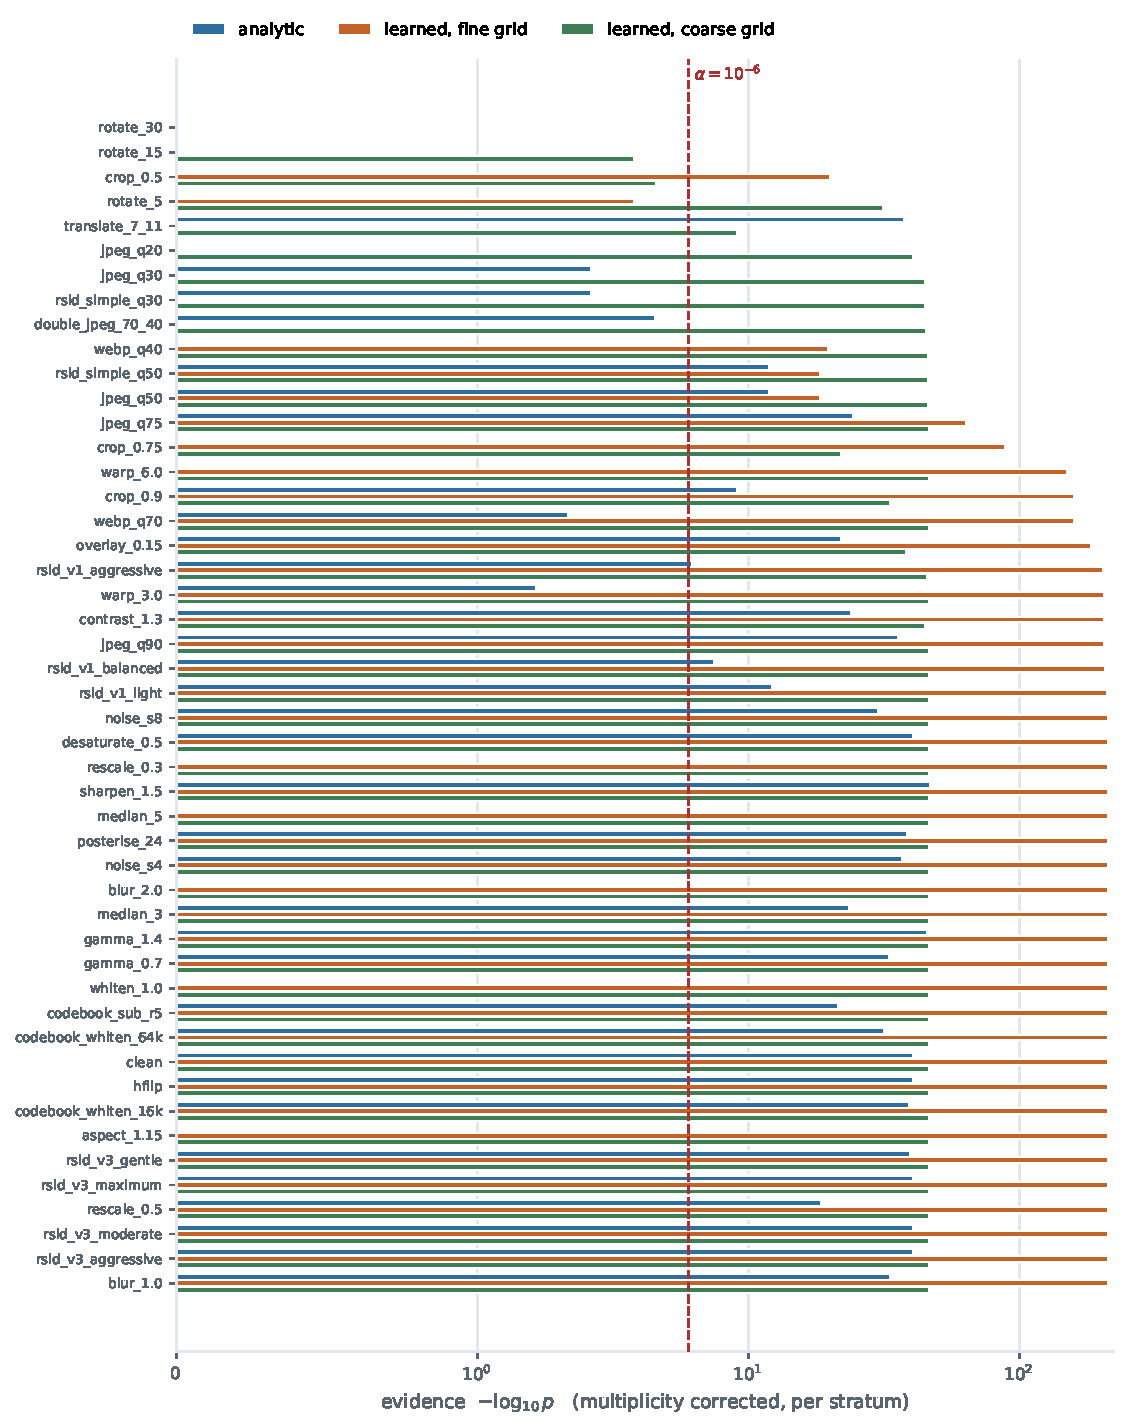
\includegraphics[width=0.94\linewidth]{../results/figures/fig15_strata_roles.pdf}
\caption{Which stratum carries which attack, ordered so the attacks with least
to spare come first. A row where one bar clears the line alone is an attack
only one stratum survives, and those rows are the whole case for carrying more
than one. The division of labour is not arbitrary: translation is carried by the
analytic stratum, whose invariance to it is proved rather than trained, while
the regeneration attacks that erase any linear spectral mark are carried by the
learned grids.}
\label{fig:strata}
\end{figure*}

\begin{figure*}[t]
\centering
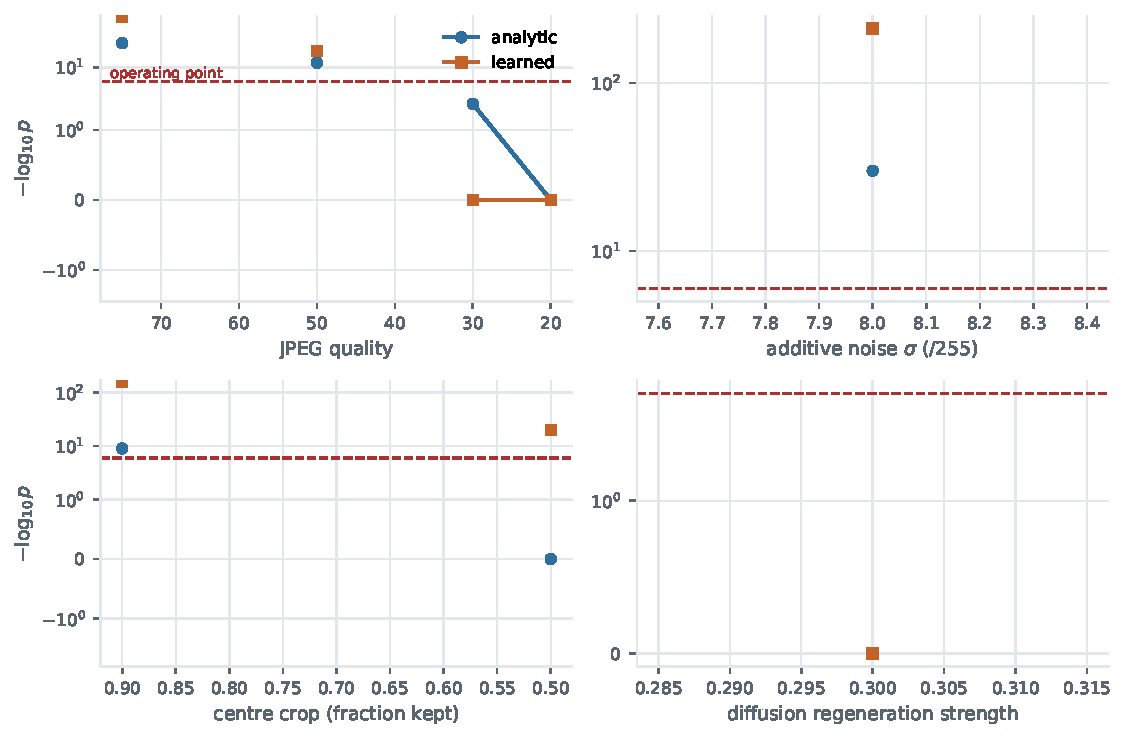
\includegraphics[width=0.92\linewidth]{../results/figures/fig03_strength_curves.pdf}
\caption{Evidence against attack strength for four families, per stratum, with
the operating point drawn. Historical pilot curves show both complementary
survival and conditions in which neither stratum remains above threshold.}
\label{fig:curves}
\end{figure*}

\begin{figure}[t]
\centering
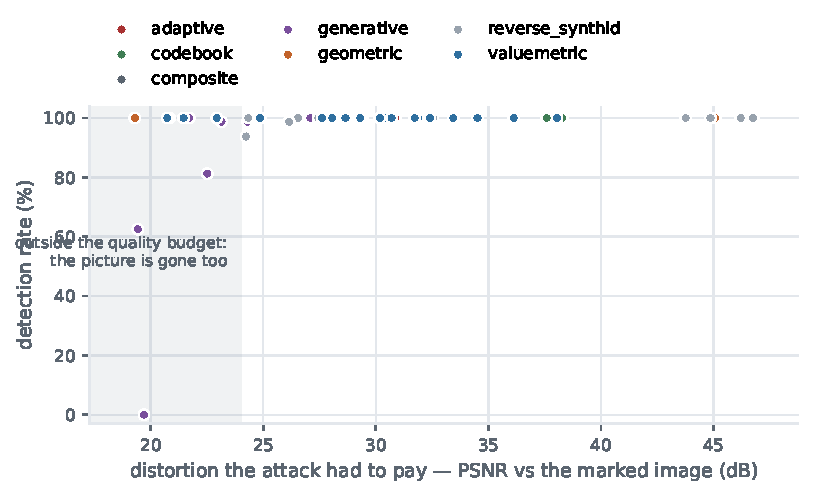
\includegraphics[width=\linewidth]{../results/figures/fig08_quality_frontier.pdf}
\caption{Detection against the distortion the attack had to pay. The shaded
region is outside the quality budget: attacks there have removed the picture, not
the mark.}
\label{fig:frontier}
\end{figure}

\section{Limitations}
\label{sec:limitations}

\paragraph{Rotation is the frontier, and we can say where it is.} The analytic
stratum cannot survive rotation at all. A rotation inside a fixed rectangular
frame is not a rotation of the signal the DFT sees: the wrap-around
discontinuities change completely, and the resulting broadband energy swamps a
per-bin perturbation. Widening its search does not help, which is the clearest
statement of the point --- with the bank extended to $\pm45^\circ$ in
one-degree steps, so that the correct angle is certainly present, a
five-degree rotation still reads $2.96$ against a clean-image $14.95$. Rotation
is therefore carried by the learned grids alone, by resynchronising: search the
angle, apply the inverse, decode. Measured on the deployed system over the full
corpus:

\begin{center}\small
\begin{tabular}{lrrr}
\toprule
rotation & $5^\circ$ & $15^\circ$ & $30^\circ$ \\
detection rate & \rotFive\% & \rotFifteen\% & \rotThirty\% \\
\bottomrule
\end{tabular}
\end{center}

Three controls establish that this is a property of the code rather than of the
detector. Supplying the exactly correct hypothesis by hand, with no crop and no
zoom, reproduces the same numbers. The full bank of \nhypotheses{} hypotheses
moves the statistic at $30^\circ$ from $6.30$ to $6.38$, so the coarse bank
already identifies the relevant neighbourhood. Refining the angle in one-degree
steps around the winner lifts a
five-degree rotation from $6.5$ to $17.1$ while doing nothing at thirty, which
exhausts alignment precision as an explanation.

The contrast with the crop axis is the argument in miniature. On the same
system, the same corpus and the same operating point, centre crops keeping
$90\%$, $75\%$ and $50\%$ of the frame are detected at \cropNine\%,
\cropSevenFive\% and \cropFive\% respectively: the crop ladder is flat exactly
where the rotation curve falls away, and the two are set by one parameter.

What remains is that a positional code cannot be read back through the
resampling that a large rotation and its inverse impose, once the cells are
small enough. That is the trade of \S\ref{sec:grids}, and carrying two grids
(Figure~\ref{fig:geometry}) buys the range neither has alone --- rotations to
\bestRot$^\circ$ and crops to \bestCrop{} of the frame --- for one extra term in
the fused minimum.

It does not buy an unbounded range, and the reason is a floor rather than a
tuning failure. Coarsening the grid further to survive larger angles costs bits
quadratically, and a statistic cannot exceed the square root of the bits it
reads: a $8\times8$ grid tops out at $64$ bits and so at a statistic of $8$,
which is below the operating threshold before any attack has been applied. At
a canonical frame of $256$ pixels the coarsest usable grid is therefore already
close to the one \sigil{} ships, and rotations far beyond the measured frontier
are out of reach for a positional code at this frame size --- not for this
implementation of one. Decoupling the two by enlarging the canonical frame,
which raises cell size without spending bits, is the direction that remains ---
though not for free: the networks are scale-sensitive, and a stratum trained at
one frame size does not transfer to another, collapsing to chance on an
untouched image. It would have to be trained there.

\paragraph{Content anchors have finite entropy.} An adversary with a very large
corpus can cluster images by descriptor and find others sharing a carrier set.
The nonce anchor closes this, but only while the learned stratum survives; an
attack that destroys the learned stratum and leaves the analytic one intact would
expose the content anchors to clustering. We are not aware of such an attack in
the suite, but the argument is structural, not empirical.

\paragraph{The guarantee is about false positives, not false negatives.}
Theorem~\ref{thm:endtoend} bounds the rate of firing on unmarked content. It says
nothing about detection rate under attack, which is measured, not proved, and
which no watermark can guarantee against an unbounded adversary --- an attacker
willing to regenerate the image from a text prompt is producing a different
image, and no mark should survive that.

\paragraph{Distortion metrics are proxies.} PSNR and SSIM under-report how
visible a structured residual is and over-report how damaging a geometric change
is. The quality budget is a defensible protocol, not a perceptual ground truth.

\section{Related work}

Spread-spectrum watermarking in a transform domain goes back to Cox et al., and
the magnitude-domain and Fourier--Mellin variants that follow it establish the
translation and RST-invariance arguments \S\ref{sec:analytic} builds on. Learned
encoder--decoder watermarks --- HiDDeN, StegaStamp and their successors ---
establish the noise-layer training recipe; the choice to put real autoencoders
and a searching opponent inside that layer, rather than a fixed menu of
differentiable approximations, is what \S\ref{sec:learned} adds. Regeneration
attacks against watermarks, and the observation that a VAE round-trip rewrites
the band a spectral mark occupies, motivate the stratification. The design
combines a search-corrected, distribution-free null upper bound with a
machine-checked proof of it, and content-derived
carriers as a stated defence against cross-image aggregation rather than an
incidental property.

\section{Conclusion}

A watermark is a statistical claim, and a claim without a calibrated error rate
is not evidence. \sigil{} makes a false-positive upper bound a design parameter,
charges honestly for every search and every fusion it performs, and proves the
core of that argument in a proof assistant. Its intended robustness comes from
carrying complementary marks and spending one budget across them. The historical
pilot results do not meet the current fidelity or corpus-size gates; the full
private-key comparison and independent null audit remain future work.

\end{document}
